\documentclass[
]{jss}

\usepackage[utf8]{inputenc}

\providecommand{\tightlist}{%
  \setlength{\itemsep}{0pt}\setlength{\parskip}{0pt}}

\author{
Nicolas Bennett\\ETH Zürich \And Drago PLecko\\ETH Zürich \And Ida-Fong Ukor\\East Kent Hospitals
}
\title{\pkg{ricu}: \proglang{R}'s interface for ICU data}

\Plainauthor{Nicolas Bennett, Drago PLecko, Ida-Fong Ukor}
\Plaintitle{ricu: R's interface for ICU data}
\Shorttitle{\pkg{ricu}: R meets ICU data}

\Abstract{
The abstract of the article.
}

\Keywords{medicine, intensive care, computational bioinformatics}
\Plainkeywords{medicine, intensive care, computational bioinformatics}

%% publication information
%% \Volume{50}
%% \Issue{9}
%% \Month{June}
%% \Year{2012}
%% \Submitdate{}
%% \Acceptdate{2012-06-04}

\Address{
    Nicolas Bennett\\
    ETH Zürich\\
    Seminar for Statistics Rämistrasse 101 CH-8092 Zurich\\
  E-mail: \email{nicolas.bennett@stat.math.ethz.ch}\\
  
      Drago PLecko\\
    ETH Zürich\\
    Seminar for Statistics Rämistrasse 101 CH-8092 Zurich\\
  E-mail: \email{drago.plecko@stat.math.ethz.ch}\\
  
      Ida-Fong Ukor\\
    East Kent Hospitals\\
    NHS University Foundation Trust William Harvey Hospital Kennington Road,
Willesborough Ashford TN24 0LZ\\
  E-mail: \email{idafong.ukor@nhs.net}\\
  
  }


% Pandoc header

\usepackage{amsmath}

\begin{document}

\hypertarget{introduction}{%
\section{Introduction}\label{introduction}}

Collection of electronic health records has seen a significant rise in
the recent years \cite{evans2016electronic}, opening up an opportunities
for a large body of data-driven research oriented towards improving
patient care and outcomes, together with helping clinicians in
decision-making \cite{jiang2017artificial}.

One example of a problem that has received much attention from the
machine learning community is early prediction of sepsis in ICU
\cite{desautels2016prediction, nemati2018interpretable, futoma2017improved, kam2017learning}.
Interestingly, there is evidence that a large proportion of the
publications are based on the same dataset \cite{fleuren2019machine},
the Medical Information Mart for Intensive Care (MIMIC)
\cite{johnson2016mimic}, which shows a systematic lack of external
validation. Part of this problem might well be the lack of a
computational infrastructure handling multiple datasets. The MIMIC-III
dataset consists of 26 different tables containing about 20GB of data.
While much work and care has gone into data preprocessing in order to
provide a self-contained ready to use data resource with MIMIC,
seemingly simple tasks such as computing a SOFA score for patients
\citep{vincent1996sofa}, remains a non trivial effort. This is only
exacerbated when aiming to co-integrate multiple different datasets of
this form is, spanning hospitals and even countries in order to capture
effects of differing practice and demographics.

The aim of the \pkg{ricu} package is to provide computational
infrastructure allowing users to access complex research questions as
easily as possible. The package also aims to enable users to write
dataset-agnostic code which can simplify implementation and shorten the
necessary time for prototyping code to different datasets. In
particular, the package handles three large, publicly available
intensive care databases: the already mentioned MIMIC-III database from
the Beth Israel Deaconess Medical Center in Boston, Massachusetts, the
eICU Collaborative Research Database \cite{pollard2018eicu}, containing
data collected from 208 hospitals across the United States, and the
HiRID database \cite{faltys2020hirid} from the Department of Intensive
Care Medicine of the Bern University Hospital, Switzerland. Together
with this, much of the functionality used is also aimed to accommodate
for addition of possible additional datasets, provided by the user. The
work most similar to ours is that of \cite{adibuzzaman2016closing} and
\cite{wang2020mimic}. However, these works address only the MIMIC-III
dataset and do not have an emphasis on dataset inter-operability.

The structure of the manuscript is as follows. In Section
\ref{implementation} we outline the different types of data useful for
research related to intensive care medicine. We explain the most
important parts of the package functionality which are used to handle
the different data types. In Section \ref{examples} we provide simple
examples which illustrate how some simple research questions can be
explored in only a couple of lines of code.

\hypertarget{implementation}{%
\section{Implementation}\label{implementation}}

In this Section we go over the categories of data useful for research
problems related to intensive care medicine. The categories we define
are fairly broad and somewhat loosely defined, as this is not the main
focus of the manuscript.

\hypertarget{physiological-data}{%
\subsection{Physiological data}\label{physiological-data}}

Labs, vitals. Could introduce the \code{ts_tbl} here.

\hypertarget{treatment-related-information}{%
\subsection{Treatment-related
information}\label{treatment-related-information}}

Antibiotics, vasopressors, mechanical ventilation\ldots{} could
introduce the \code{win_tbl} here.

\hypertarget{co-morbidities}{%
\subsection{Co-morbidities}\label{co-morbidities}}

Based on ICD-9 codes. Should enable the extraction of co-morbidities
used for the Charlson and Elixhauser scores.

\hypertarget{admission-diagnoses}{%
\subsection{Admission diagnoses}\label{admission-diagnoses}}

Categorizing into surgical, non-surgical and other might be sufficient
for now.

\hypertarget{patient-information}{%
\subsection{Patient information}\label{patient-information}}

Age, gender, other demograpichs, patient stay information.

\hypertarget{outcomes}{%
\subsection{Outcomes}\label{outcomes}}

Death outcome, prolonged ICU stay outcome.

\hypertarget{examples}{%
\section{Examples}\label{examples}}

We focus on two simple examples with which we try to cover most of the
data types described in Section \ref{implementation}.

\hypertarget{lactate-and-mortality}{%
\subsection{Lactate and mortality}\label{lactate-and-mortality}}

The first example we look at is the association of lactate levels and
mortality. This problem has been studied before and it is widely
accepted that both static and dynamic lactate indices are associated
with increased mortality
\citep{haas2016severe, nichol2011dynamic, van2013cumulative}. We quickly
look at how one might fit a time-varying proportional hazards Cox model
\citep{therneau2015package} in order to investigate this problem. We
additionally include the Sequential Organ Failure Assessment (SOFA)
score \citep{vincent1996sofa} as a general predictor of illness
severity.

\begin{CodeChunk}

\begin{CodeInput}
R> source <- "mimic_demo"
R> # data loading
R> tbl <- load_concepts(c("lact", "death", "sofa"), source,
+                      verbose = FALSE)
\end{CodeInput}

\begin{CodeOutput}
Only concept data from a single data source can be loaded a the time. Please
choose one of mimic_demo
\end{CodeOutput}

\begin{CodeOutput}
Data aggregation cannot be disabled (i.e. passing an `aggregate` value of
`FALSE` for at least one concept) when data merging is enabled.
\end{CodeOutput}

\begin{CodeOutput}
No overlap between configured id var options and available columns for table
`labevents` in mimic_demo
\end{CodeOutput}

\begin{CodeOutput}
index is not compatible with an interval of 1 mins
\end{CodeOutput}

\begin{CodeOutput}
cannot mix interval lengths when row-binding
\end{CodeOutput}

\begin{CodeOutput}
For automatically determining an aggregation function, either all of or none of
vars `lact` are expected to be of numeric type
\end{CodeOutput}

\begin{CodeOutput}
No overlap between configured id var options and available columns for table
`admissions` in mimic_demo
\end{CodeOutput}

\begin{CodeOutput}
No overlap between configured id var options and available columns for table
`labevents` in mimic_demo
\end{CodeOutput}

\begin{CodeOutput}
index is not compatible with an interval of 1 mins
\end{CodeOutput}

\begin{CodeOutput}
cannot mix interval lengths when row-binding
\end{CodeOutput}

\begin{CodeOutput}
removed 32 (2.77%) of rows due to out of range entries
\end{CodeOutput}

\begin{CodeOutput}
not all units are in [mmHg]: mm Hg (99.82%), MM HG (0.18%)
\end{CodeOutput}

\begin{CodeOutput}
No overlap between configured id var options and available columns for table
`labevents` in mimic_demo
\end{CodeOutput}

\begin{CodeOutput}
index is not compatible with an interval of 1 mins
\end{CodeOutput}

\begin{CodeOutput}
cannot mix interval lengths when row-binding
\end{CodeOutput}

\begin{CodeOutput}
removed 4 (1.18%) of rows due to out of range entries
\end{CodeOutput}

\begin{CodeOutput}
not all units are in [%]: NA (18.26%)
\end{CodeOutput}

\begin{CodeOutput}
cannot mix interval lengths when row-binding
cannot mix interval lengths when row-binding
\end{CodeOutput}

\begin{CodeOutput}
multiple units detected: . (0.04%), cmH2O (48.08%), L/min (11.22%), mL
(10.09%), ml/B (11.38%), sec (2.79%), NA (16.4%)
\end{CodeOutput}

\begin{CodeOutput}
cannot mix interval lengths when row-binding
\end{CodeOutput}

\begin{CodeOutput}
multiple units detected: None (0.93%), NA (99.07%)
\end{CodeOutput}

\begin{CodeOutput}
x is not a `difftime` object
\end{CodeOutput}

\begin{CodeOutput}
No overlap between configured id var options and available columns for table
`labevents` in mimic_demo
\end{CodeOutput}

\begin{CodeOutput}
index is not compatible with an interval of 1 mins
\end{CodeOutput}

\begin{CodeOutput}
cannot mix interval lengths when row-binding
\end{CodeOutput}

\begin{CodeOutput}
removed 3 (0.19%) of rows due to out of range entries
\end{CodeOutput}

\begin{CodeOutput}
No overlap between configured id var options and available columns for table
`labevents` in mimic_demo
\end{CodeOutput}

\begin{CodeOutput}
index is not compatible with an interval of 1 mins
\end{CodeOutput}

\begin{CodeOutput}
cannot mix interval lengths when row-binding
\end{CodeOutput}

\begin{CodeOutput}
index is not compatible with an interval of 1 mins
\end{CodeOutput}

\begin{CodeOutput}
cannot mix interval lengths when row-binding
\end{CodeOutput}

\begin{CodeOutput}
removed 35 (0.22%) of rows due to out of range entries
\end{CodeOutput}

\begin{CodeOutput}
cannot mix interval lengths when row-binding
\end{CodeOutput}

\begin{CodeOutput}
removed 1 (0.26%) of rows due to out of range entries
\end{CodeOutput}

\begin{CodeOutput}
cannot mix interval lengths when row-binding
cannot mix interval lengths when row-binding
cannot mix interval lengths when row-binding
\end{CodeOutput}

\begin{CodeOutput}
index is not compatible with an interval of 1 mins
\end{CodeOutput}

\begin{CodeOutput}
cannot mix interval lengths when row-binding
\end{CodeOutput}

\begin{CodeOutput}
removed 2 (0.05%) of rows due to out of range entries
\end{CodeOutput}

\begin{CodeOutput}
index is not compatible with an interval of 1 mins
\end{CodeOutput}

\begin{CodeOutput}
cannot mix interval lengths when row-binding
\end{CodeOutput}

\begin{CodeOutput}
removed 5 (0.13%) of rows due to out of range entries
\end{CodeOutput}

\begin{CodeOutput}
index is not compatible with an interval of 1 mins
\end{CodeOutput}

\begin{CodeOutput}
cannot mix interval lengths when row-binding
\end{CodeOutput}

\begin{CodeOutput}
removed 7 (0.18%) of rows due to out of range entries
\end{CodeOutput}

\begin{CodeOutput}
index is not compatible with an interval of 1 mins
\end{CodeOutput}

\begin{CodeOutput}
cannot mix interval lengths when row-binding
\end{CodeOutput}

\begin{CodeOutput}
removed 2 (0.1%) of rows due to out of range entries
\end{CodeOutput}

\begin{CodeOutput}
index is not compatible with an interval of 1 mins
\end{CodeOutput}

\begin{CodeOutput}
cannot mix interval lengths when row-binding
\end{CodeOutput}

\begin{CodeOutput}
x is not a `difftime` object
\end{CodeOutput}

\begin{CodeOutput}
x does not contain column `icustay_id`
\end{CodeOutput}

\begin{CodeOutput}
cannot mix interval lengths when row-binding
\end{CodeOutput}

\begin{CodeOutput}
x is not a `difftime` object
\end{CodeOutput}

\begin{CodeOutput}
x does not contain column `icustay_id`
\end{CodeOutput}

\begin{CodeOutput}
cannot mix interval lengths when row-binding
\end{CodeOutput}

\begin{CodeOutput}
x is not a `difftime` object
x is not a `difftime` object
\end{CodeOutput}

\begin{CodeOutput}
x does not contain column `icustay_id`
\end{CodeOutput}

\begin{CodeOutput}
x is not a `difftime` object
\end{CodeOutput}

\begin{CodeOutput}
No overlap between configured id var options and available columns for table
`labevents` in mimic_demo
\end{CodeOutput}

\begin{CodeOutput}
index is not compatible with an interval of 1 mins
\end{CodeOutput}

\begin{CodeOutput}
cannot mix interval lengths when row-binding
\end{CodeOutput}

\begin{CodeOutput}
removed 2 (0.12%) of rows due to out of range entries
\end{CodeOutput}

\begin{CodeOutput}
index is not compatible with an interval of 1 mins
\end{CodeOutput}

\begin{CodeOutput}
cannot mix interval lengths when row-binding
\end{CodeOutput}

\begin{CodeOutput}
removed 21 (0.23%) of rows due to out of range entries
\end{CodeOutput}

\begin{CodeOutput}
not all units are in [mL]: NA (0.08%)
\end{CodeOutput}

\begin{CodeOutput}
x is not a `difftime` object
x is not a `difftime` object
x is not a `difftime` object
\end{CodeOutput}

\begin{CodeOutput}
x does not contain column `icustay_id`
\end{CodeOutput}

\begin{CodeOutput}
x is not a `difftime` object
x is not a `difftime` object
\end{CodeOutput}

\begin{CodeOutput}
x does not contain column `icustay_id`
\end{CodeOutput}

\begin{CodeOutput}
cannot mix interval lengths when row-binding
\end{CodeOutput}

\begin{CodeOutput}
x is not a `difftime` object
\end{CodeOutput}

\begin{CodeOutput}
x does not contain column `icustay_id`
\end{CodeOutput}

\begin{CodeOutput}
cannot mix interval lengths when row-binding
\end{CodeOutput}

\begin{CodeOutput}
x is not a `difftime` object
\end{CodeOutput}

\begin{CodeOutput}
x does not contain column `icustay_id`
\end{CodeOutput}

\begin{CodeOutput}
cannot mix interval lengths when row-binding
\end{CodeOutput}

\begin{CodeOutput}
x is not a `difftime` object
\end{CodeOutput}

\begin{CodeOutput}
x does not contain column `icustay_id`
\end{CodeOutput}

\begin{CodeOutput}
cannot mix interval lengths when row-binding
\end{CodeOutput}

\begin{CodeOutput}
x is not a `difftime` object
\end{CodeOutput}

\begin{CodeOutput}
x does not contain column `icustay_id`
\end{CodeOutput}

\begin{CodeOutput}
cannot mix interval lengths when row-binding
\end{CodeOutput}

\begin{CodeOutput}
x is not a `difftime` object
\end{CodeOutput}

\begin{CodeOutput}
x does not contain column `icustay_id`
\end{CodeOutput}

\begin{CodeOutput}
cannot mix interval lengths when row-binding
\end{CodeOutput}

\begin{CodeOutput}
x is not a `difftime` object
\end{CodeOutput}

\begin{CodeOutput}
x does not contain column `icustay_id`
\end{CodeOutput}

\begin{CodeOutput}
cannot mix interval lengths when row-binding
\end{CodeOutput}

\begin{CodeOutput}
x is not a `difftime` object
\end{CodeOutput}

\begin{CodeOutput}
x does not contain column `icustay_id`
\end{CodeOutput}

\begin{CodeOutput}
cannot mix interval lengths when row-binding
\end{CodeOutput}

\begin{CodeOutput}
x is not a `difftime` object
x is not a `difftime` object
x is not a `difftime` object
\end{CodeOutput}

\begin{CodeOutput}
x does not contain column `icustay_id`
\end{CodeOutput}

\begin{CodeOutput}
x is not a `difftime` object
x is not a `difftime` object
\end{CodeOutput}

\begin{CodeOutput}
x does not contain column `icustay_id`
\end{CodeOutput}

\begin{CodeOutput}
cannot mix interval lengths when row-binding
\end{CodeOutput}

\begin{CodeInput}
R> tbl <- tbl[, c(meta_vars(tbl), "lact", "sofa", "death"), with = FALSE]
R> tbl <- tbl[, lact := nafill(lact, "locf")]
R> tbl <- tbl[, lact := nafill(lact, fill = 1)]
R> tbl[, event := as.integer(sum(death, na.rm = TRUE) > 0), by = c(id_vars(tbl))]
R> tbl[, event := last_event(event), by = c(id_vars(tbl))]
R> tbl[, next_charttime := charttime+1L]
R> # model fitting
R> cox_time_mod <- coxph(
+   Surv(charttime, next_charttime, event) ~ lact + sofa,
+   data = tbl
+ )
\end{CodeInput}
\end{CodeChunk}

We visualize the results of the model

\begin{CodeChunk}


\begin{center}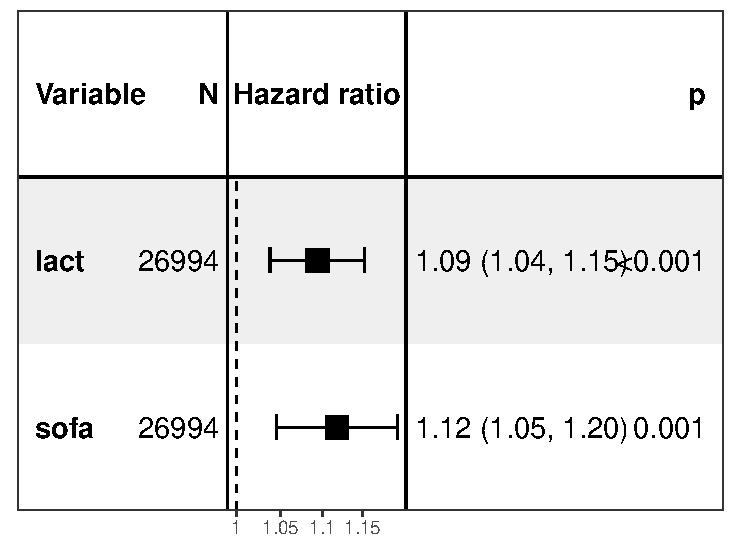
\includegraphics{/tmp/RtmplUiibd/file3dc86fe260e/dev/articles/jss_files/figure-latex/cox_plot-1} \end{center}

\end{CodeChunk}

A simple exploration already shows that the increased values of lactate
are associated with mortality, even after adjusting for the SOFA score.

\hypertarget{diabetes-and-insulin-treatment}{%
\subsection{Diabetes and insulin
treatment}\label{diabetes-and-insulin-treatment}}

The next example we turn to covers the usage of co-morbidities and
treatment related information. We look at the amount of insulin
administered to patients in the first 24 hours from their ICU admission.
In particular, we investigate if patients who are diabetic receive more
insulin in the first day of their stay. We extract the data as follows:

\begin{CodeChunk}

\begin{CodeInput}
R> source <- "mimic_demo"
R> ins_breaks <- c(0.01, 10, 20, 30, 40)
R> 
R> cohort <- stay_windows(source)
R> ins_treat <- load_concepts("ins", source, verbose = FALSE)
\end{CodeInput}

\begin{CodeOutput}
Only concept data from a single data source can be loaded a the time. Please
choose one of mimic_demo
\end{CodeOutput}

\begin{CodeOutput}
Data aggregation cannot be disabled (i.e. passing an `aggregate` value of
`FALSE` for at least one concept) when data merging is enabled.
\end{CodeOutput}

\begin{CodeOutput}
x is not a `difftime` object
\end{CodeOutput}

\begin{CodeOutput}
cannot mix interval lengths when row-binding
\end{CodeOutput}

\begin{CodeOutput}
removed 1037 (32.17%) of rows due to out of range entries
\end{CodeOutput}

\begin{CodeOutput}
multiple units detected: Uhr (66.16%), units/hr (33.84%)
\end{CodeOutput}

\begin{CodeOutput}
For automatically determining an aggregation function, either all of or none of
vars `ins` are expected to be of numeric type
\end{CodeOutput}

\begin{CodeInput}
R> ins_treat <- ins_treat[get(index_var(ins_treat)) <= 24L]
R> 
R> ins_treat <- ins_treat[,
+   list(ins_sum = .bincode(sum(ins), breaks = c(-Inf, ins_breaks, Inf)) - 1),
+   by = c(id_vars(ins_treat))
+ ]
\end{CodeInput}

\begin{CodeOutput}
x is not a `difftime` object
\end{CodeOutput}

\begin{CodeInput}
R> cohort <- merge(cohort, ins_treat, by = id_vars(cohort), all.x = TRUE)
R> cohort[, Diabetic := get(id_vars(cohort)) %in% diabetes(source)]
\end{CodeInput}

\begin{CodeOutput}
No overlap between configured id var options and available columns for table
`diagnoses_icd` in mimic_demo
\end{CodeOutput}

\begin{CodeInput}
R> cohort[is.na(ins_sum), "ins_sum"] <- 0
\end{CodeInput}
\end{CodeChunk}

After this, we can visualize the difference between the two groups with
a histogram:

\begin{CodeChunk}


\begin{center}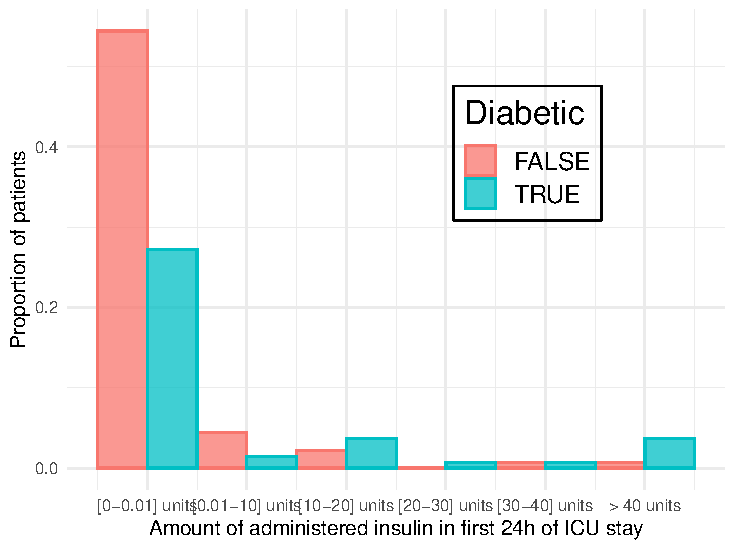
\includegraphics{/tmp/RtmplUiibd/file3dc86fe260e/dev/articles/jss_files/figure-latex/diabetes_visualize-1} \end{center}

\end{CodeChunk}

The plot might suggest that diabetic patients do receive more insulin
that non-diabetic patients, in the first day of ICU stay.

\bibliography{jss.bib}


\end{document}

